\documentclass{standalone}
\usepackage{tikz}
\usetikzlibrary{matrix,chains,positioning,decorations.pathreplacing,arrows}

\begin{document}

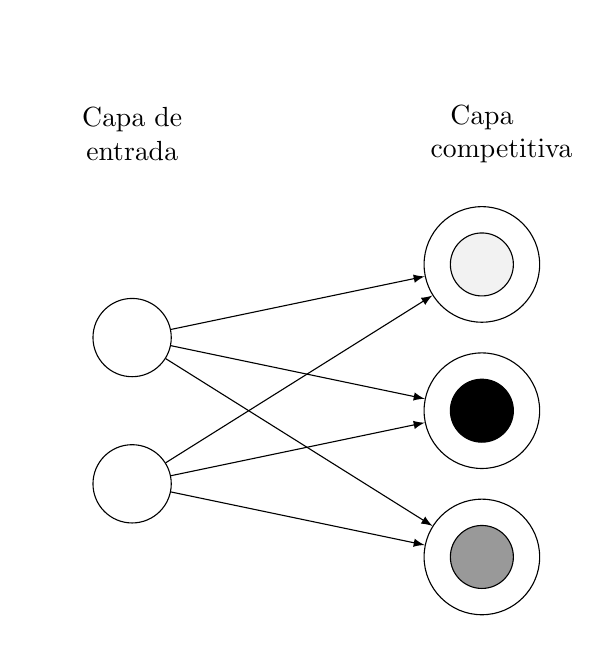
\begin{tikzpicture}[
plain/.style={
  draw=none,
  fill=none,
  },
net/.style={
  matrix of nodes,
  nodes={
    draw,
    circle,
    inner sep=10pt
    },
  nodes in empty cells,
  column sep=2cm,
  row sep=-9pt
  },
>=latex
]
\matrix[net] (mat)
{
|[plain]| \parbox{1.3cm}{\centering Capa de\\ entrada} & |[plain]| \parbox{1.3cm}{\centering Capa\\ competitiva} \\
|[plain]| & $\mathbf{w}_1$ \\
  & |[plain]| \\
 |[plain]| & $\mathbf{w}_2$  \\
& |[plain]| \\
|[plain]| & $\mathbf{w}_3$ \\
};
\foreach \ai in {3,5}
{\foreach \aii in {2,4,6}
  \draw[->] (mat-\ai-1) -- (mat-\aii-2);
}

\draw [fill=black!5] (mat-2-2) circle [radius=0.4];
\draw [fill=black] (mat-4-2) circle [radius=0.4];
\draw [fill=black!40] (mat-6-2) circle [radius=0.4];


\end{tikzpicture}


\end{document}